\setchapterpreamble[u]{\margintoc}
\chapter{Numeri e approssimazioni}
\labch{numbers}

\section{Introduzione: Numeri}

La rappresentazione numerica a cui il calcolo scientifico fa riferimento principalmente
è quella dei numeri reali; nell’ambito informatico tale rappresentazione utilizza
il concetto di numeri a virgola mobile come standard: i numeri reali vengono
rappresentati attraverso una notazione scientifica in base due tramite la seguente formula:

$$
	(-1)^S \left( 1 + \sum_n M_n 2^{-n} \right) \cdot 2^{E}
$$

Dove:
\begin{description}
	\item $S$ è il valore booleano per il \textbf{segno}
	\item $M$ è la parte decimale detta \textbf{mantissa}

	\item $E = e - d$ è l'\textbf{esponente} con $d$ (offset), $e$ (esponente dopo offset)
\end{description}

\section{Esercizi}

\subsection{Precisione}

\paragraph{Nozioni teoriche}

\subparagraph{Definizione} La \textit{precisione di macchina} (o \textit{$\epsilon$ di macchina})
è la differenza tra 1 e il numero successivo rappresentabile dato il numero di bit
richiesti, esso sarà dunque:

$$
	\epsilon = 2^{-M}
$$

Nello standard dei numeri a virgola mobile (IEE 754) si studiano principalmente
due sottoclassi di numeri i cui nominativi nei linguaggi C-like sono:

\begin{description}
	\item[float] numero a singola precisione (32 bit di memoria):
		\begin{itemize}
			\item $M$: 23 bit
			\item $E$: 8 bit
			\item Valore massimo: $3.40 \cdot 10^{38}$
			\item $\epsilon$: $\sim 10^{-7}$
		\end{itemize}
	\item[double] numero a doppia precisione (64 bit di memoria):
		\begin{itemize}
			\item $M$: 52 bit
			\item $E$: 11 bit
			\item Valore massimo: $1.8 \cdot 10^{308}$
			\item $\epsilon$: $\sim 10^{-16}$
		\end{itemize}

\end{description}

\paragraph{Richiesta} Scriverete un programma C che esegua le seguenti operazioni:

\begin{lstlisting}
    define f in single precision = 1.2e34
    for loop with 24 cycles:
        f *= 2
        print f in scientific notation
    repeat for d in double precision, starting from 1.2e304
    define d in double precision = 1e-13
    for loop with 24 cycles:
        d /= 2
        print d and 1+d in scientific notation
    repeat for single precision
\end{lstlisting}

Esaminare il range minimo e massimo e il ruolo dell'errore di macchina.

\paragraph{Implementazione e osservazioni}

\subparagraph{File necessari} sorgente: \texttt{number\_precision.c}, dati: \texttt{number\_precision.dat}

Il codice sorgente scritto utilizza funzionalità base del linguaggio C. \sidenote{
	Per formattare il codice secondo la richiesta del problema si usi la
	definizione \texttt{EXERCISE\_FORMAT}, altrimenti verrà utilizzata una formattazione
	più compatta per leggere in maniera più diretta i dati, si consiglia di utilizzare
	quest'ultima per comprendere l'analisi sottostante}

\paragraph{Analisi e conclusioni}

Dai dati ottenuti si possono notare in maniera esaustiva varie proprietà dei
numeri a virgola mobile:

\begin{enumerate}
	\item Esiste un \textit{valore massimo} sia per singola ($\sim 3 \cdot 10^{38}$) sia
	      per doppia precisione ($\sim 2 \cdot 10^{308}$), superato esso viene mostrato un
	      valore esatto \textit{inf} definito dallo standard descritto in precedenza;

	\item I numeri hanno un \textit{errore macchina} dettato dalla capienza di memoria della mantissa;

	\item Come mostrerà più precisamente la prossima sezione, l’errore viene
	      \textit{propagato} nella somma:

	      \begin{itemize}
		      \item $1 + f_{mult}$ perde completamente l’informazione su $f_{mult}$

		      \item $1 + d_{mult}$ la conserva soltanto per le prime iterazioni;
	      \end{itemize}
\end{enumerate}
\subsection{Propagazione degli errori}
\paragraph{Nozioni teoriche}

E' immediato notare come i numeri a virgola mobile possano essere rappresentati come
variaili casuali con errore associato, derivante dalla precisione di macchina.

Prendiamo in esame una funzione $f(x, y)$ dove $x, y$ sono variabili casuali indipendenti
con rispettivo errore $\sigma_x, \sigma_y$, allora l'errore su f sarà:

$$
	\sigma_f^2 = {\left( \frac{\partial f}{\partial x} \right)^2 \sigma_x^2 + \left( \frac{\partial f}{\partial y} \right)^2 \sigma_y^2}
$$

Assumendo ora $f = x + y$ otteniamo:

$$
	\sigma_f^2 = {\sigma_x^2 + \sigma_y^2}
$$

Notiamo immediatamente quindi che se $x \gg y $ allora $\sigma_f \approx \sigma_x$ quindi
si perde l'informazione su $y$ nella somma.


\paragraph{Richiesta} 

Si scriva in C un programma che esegua le seguenti operazioni:

\begin{lstlisting}
    calculate (0.7 + 0.1) + 0.3 and print 16 digits
    calculate 0.7 + (0.1 + 0.3) and print 16 digits
    define xt = 1.e20; yt = -1.e20; zt = 1
    calculate (xt + yt) + zt
    calculate xt + (yt + zt)
\end{lstlisting}

Esaminare la non-associatività dell'addizione e il ruolo degli errori di arrotondamento.



\paragraph{Implementazione e osservazioni}

\subparagraph{File necessari} sorgente: \texttt{error\_propagation.c}

In base alle richieste l'output è il seguente:

\begin{enumerate}

	\item $(0.7 + 0.1) + 0.3 =_? 0.7 + (0.1 + 0.3)$:
	      $$\texttt{Output: 1.1000000238418579, 1.1000000238418579}$$

	      La somma risulta associativa.

	\item $[10^{20} + (-10^{20})] + 1 =_? 10^{20} + [(-10^{20}) + 1]$:
	      $$\texttt{Output: 1.0000000000000000, 0.0000000000000000}$$

	      La somma risulta non associativa.
\end{enumerate}

\label{sec:propagation}
\paragraph{Analisi}

Utilizzando le formule discusse si può studiare la propagazione dell’errore nella somma.
In essa la propagazione dipende dall’errore assoluto dei singoli addendi.
Assumendo numeri a singola precisione e ricordando che $ \sigma_x \approx \epsilon \sim 10^{-7}$,
si ottengono i seguenti casi:

\begin{enumerate}

	\item Per i valori 0.7, 0.1, 0.3 l’ordine di grandezza è lo stesso, quindi,
	      tutti i valori possegono un errore assoluto $\Delta x \sim 10^{-8}$; propagando
	      l’errore nella somma si ottiene dunque $\Delta_{output} \sim 3 \cdot \Delta x$ in accordo con
	      i risultati.

	\item Il risultato è describile come un caso limite nell’errore di propagazione rispetto
	      alla singola precisione, infatti, $10^{20}$ avrà un errore assoluto di $\sim 10^{13}$
	      mentre 1 di $10^{-7}$!

	      La spiegazione dell'output ottenuto, dunque, si basa sulla differenza
	      tra ordini di grandezza dei diversi addendi:
	      \begin{itemize}
		      \item Nel termine a sinistra
		            vengono sommati prima numeri con errore assoluto paragonabile.
		            Si ottiene quindi $\sim 0$ che sarà poi sommato con un numero
		            avente errore assoluto simile a 1.

		      \item
		            Nel termine a destra, invece, si sommano due valori con venti
		            ordini di grandezza di differenza: l’errore assoluto di
		            $10^{20}$ prevale e si perde qualsiasi informazione nella somma per termini:
		            $$x \ll 10^{20} \Rightarrow x + 10^{20} \sim 10^{20}$$
		            Segue che $\mathit{1}$ sarà ignorato nella somma a destra.
	      \end{itemize}

\end{enumerate}

\paragraph{Conclusioni}
Nel manipolare numeri in un calcolatore l’operazione eseguita, la precisione e
la differenza in ordine di grandezza dei numeri partecipanti devono essere tenuti
sempre in considerazione specialmente nelle addizioni.

\setchapterpreamble[u]{\margintoc}
\chapter{Approssimazioni}
\labch{approx}



\section{Introduzione}

Le approssimazioni di funzioni rivestono un ruolo fondamentale in ambito scientifico,
specialmente nella fisica computazionale, dove spesso non è possibile risolvere
esattamente le equazioni che descrivono i fenomeni fisici.

Queste approssimazioni permettono di semplificare funzioni complesse attraverso
metodi numerici, rendendo più accessibile la loro analisi e il calcolo delle
soluzioni.
Tali tecniche consentono di ottenere stime accurate di grandezze fisiche che
altrimenti sarebbero difficili da trattare analiticamente, con una precisione
dipendente dalla complessità del modello e dalla quantità di risorse computazionali
disponibili.

Alcuni dei metodi più comuni includono l'approssimazione polinomiale: tra cui
le serie di Taylor, argomento di questa sezione; o tecniche come l'interpolazione
che sarà l'argomento della sezione pertinente.

\section{Esercizi}


\subsection{Funzione esponenziale}

\paragraph{Nozioni teoriche}

La funzione esponenziale è esprimibile in serie di McLaurin come:

$$
	e^x = \sum_{n=0} \frac{x^n}{n!} + \epsilon
$$

dove $\epsilon$ rappresenta l'errore commesso nell'approssimare la funzione:

$$
	\epsilon \approx \frac{x^{n+1}}{(n+1)!}
$$

ove $n$ è il grado della serie di Taylor.

\paragraph{Richiesta}

Si consideri la funzione \( f(x) = \exp(x) \) nell'intervallo \( x \in [0.1, 1] \).

Scrivere un programma in C che calcoli il fnzionale di approssimazione corrispondente (in doppia precisione)
\[
g_n(x) = \sum_{i=0}^{n} \frac{x^i}{i!}
\]

\begin{enumerate}
    \item Verificare che l'errore scala approssimativamente come \( \frac{x^{n+1}}{(n+1)!} \) per \( n = 1, 2, 3, 4 \).
    \item L'errore \( \left| f(x) - g(x) \right| \), nell'intervallo dato in \( x \), differisce da \( \frac{x^{n+1}}{(n+1)!} \): perché e per quali valori di \( x \)?
\end{enumerate}


\paragraph{Implementazione e osservazioni}

% file necessari
\subparagraph{File necessari} sorgente: \texttt{exp\_approx.c}, dati: \texttt{exp\_approx\_$n$.dat} \\ $n = 1, 2, 3, 4$

\begin{marginfigure}
    \hspace*{-2cm}
	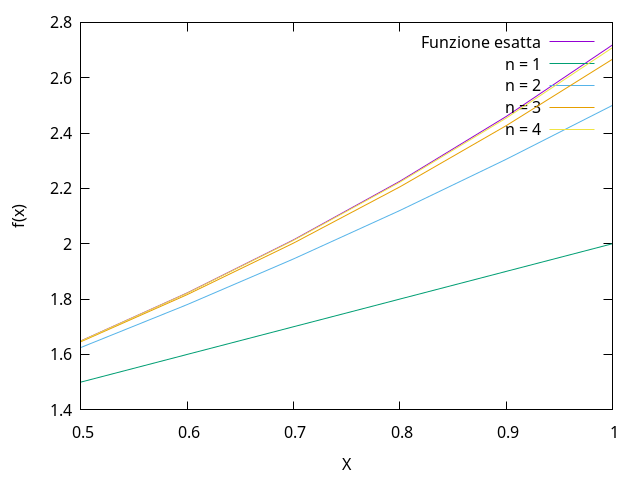
\includegraphics[width=1.5\textwidth]{exp_confront.png}
	\caption{Confronto tra funzione esponenziale e la n-esima approssimazione}
	\labfig{expfunc}
\end{marginfigure}


\begin{marginfigure}
    \hspace*{-2cm}
	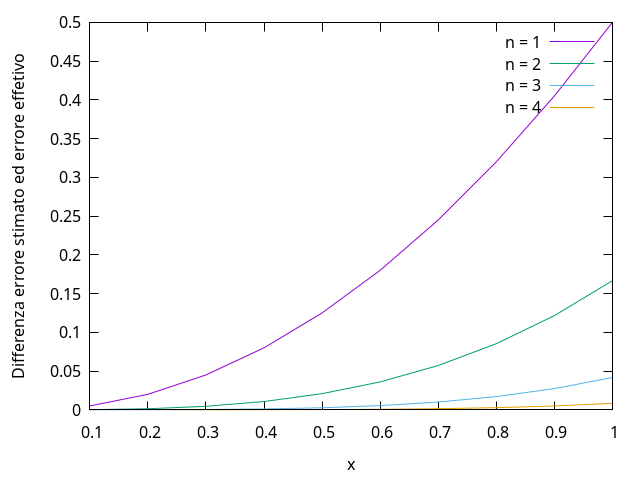
\includegraphics[width=1.5\textwidth]{error_diff_n.png}
	\caption{Differenza tra errore teorico ed errore ottenuto}
	\labfig{errordiff}
\end{marginfigure}

La funzione esponenziale ottenuta approssimando si può osservare in \reffig{expfunc}.

\begin{enumerate}
	\item L'errore scala effettivamente come $\frac{x^{n+1}}{(n+1)!}$ per valori
	      vicini a 0 e per valori di n maggiori, come si può osservare in \reffig{errordiff}.

	\item Sempre dalla \reffig{errordiff} si può notare come l'errore aumenti all'allontanarsi
	      da x = 0 e cominci a differire dall'errore teorico.
	      Ciò si intuscisce studiando la condizione per cui continui $\epsilon_{teorico} \approx \epsilon_{reale}$ è
	      soddisfatta: 
          $$O(x^n) \rightarrow o(x^{n+1}) \rightarrow \epsilon_{teorico} \ll 1$$ 
          La condizione dipende
	      da $n$ e $x$: per valori bassi di $n, x^n$ prevale sul fattoriale e la differenza
	      da $\epsilon_{teorico}$ è maggiormente visibile. Come si può vedere in \reffig{errordiff}
	      per $n = 4$ e l'errore tende a 0 molto più velocemente.

\end{enumerate}

% NOTE: la differenza dall'errore teorico aumenta all'allontanarsi da x = 0 poiche'
% la serie di taylor e' stata espansa in x = 0

\subsection{Problema di Basilea}

\paragraph{Nozioni teoriche}

Il problema di Basilea consiste nel calcolare il valore della serie armonica generalizzata:

$$
	S(N) = \sum_{n=1}^{N} \frac{1}{n^2} \xrightarrow{N \to \infty} \zeta(2) = \frac{\pi^2}{6}
$$

\paragraph{Richiesta} 

Calcolare la seguente somma

\[
\sum_{n=1}^{\infty} \frac{1}{n^2} = \frac{\pi^2}{6} = \lim_{N \to \infty} S(N)
\]

con

\[
S(N) = \sum_{n=1}^{N} \frac{1}{n^2}
\]

\begin{enumerate}
    \item Calcolare la somma in precisione singola usando l'ordine normale \( n = 1, 2, \dots, N \)
    \item Calcolare la somma in precisione singola usando l'ordine inverso \( n = N, \dots, 2, 1 \)
    \item Studiare la convergenza di entrambe in funzione di \( N \), tracciando \( \left| S(N) - \frac{\pi^2}{6} \right| \)
    \item Ripetere i punti 1, 2 e 3 in precisione doppia
\end{enumerate}


\paragraph{Osservazioni e conclusioni}

\subparagraph{Singola precisione}

I valori ottenuti per numeri a singola precisione sono:
% due valori, somma inversa e somma diretta

$$
	S_{incr}(N) \approx \mathtt{1.6447253} \quad \text{per } N = 6000
$$

$$
	S_{inv}(N) \approx \mathtt{1.6447674} \quad \text{per } N = 6000
$$

\begin{marginfigure}%[H]
	%	\centering
    %\hspace*{-2cm}
	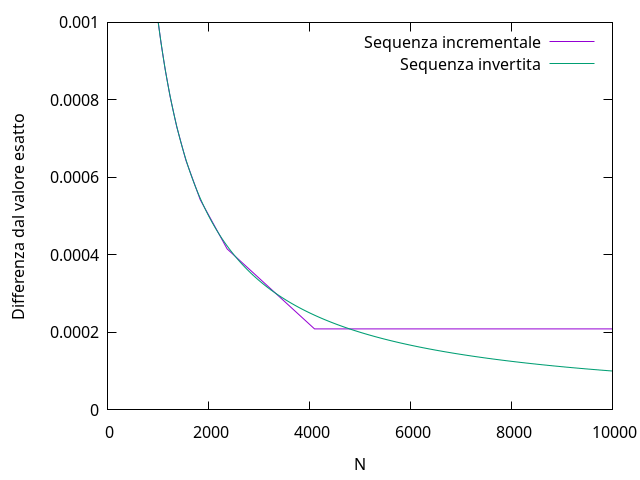
\includegraphics[width=1.5\columnwidth]{seq_inv_sum_error.png}
	\caption{$|S(N) - \pi^6 / 2|$ per valori grandi di N, si nota un singolare
		andamento della somma a partire da valori $ x \approx 4000$, \textbf{la
			stessa cosa non succede invece per numeri a doppia precisione}}
	\labfig{sumerr}
\end{marginfigure}

Il risultato è spiegabile in maniera equivalente a \ref{sec:propagation}: l'ordine
della somma conta nella propagazione di errori in numeri a virgola mobile. Infatti:
\begin{itemize}
	\item Nella somma incrementale, il valore di partenza è $1/1^2 = 1$ (il valore
	      \textit{più grande} della somma con errore $\epsilon \approx 10^{-7}$),
	      dato che la somma si propaga con gli errori assoluti degli addendi,
	      considerando $N = 4000$:

	      $$\epsilon_{tot} \approx N \epsilon \approx 4 \cdot 10^{-4}$$

	      Che è circa lo stesso ordine di grandezza in cui inizia l'andamento costante
	      della somma. Per $N > 4000$ la somma perde le informazioni su numeri piccoli
	      poichè l'errore propagato è maggiore del valore sommato.

	\item La somma invertita, invece, inizia con il valore più piccolo della serie,
	      per esempio $1/4000^2 \approx 6.25 \cdot 10^{-8}$, e propaga con errori sempre maggiori
	      ma inferiori alle cifre significative del valore successivo (più grande).
	      Ciò comporta che la perdita di informazioni non è abbastanza significativa
	      per causare errori di arrotondamento notevoli.
\end{itemize}
\subparagraph{Doppia precisione}

% TODO: probabilmente migliorare la spiegazione

In doppia precisione l'errore macchina è ancora minore e l'effetto diventa trascurabile
subentrano ulteriori errori (per numeri di $5 \cdot 10^5$) non causati dalla precisione del numero ma da limiti 
del programma scritto o del compilatore/interprete utilizzato.

In conclusione, si sottilinea, come nel capitolo precedente, l'importanza di considerare
l'ordine della somma e la precisione del calcolo in problemi numerici.










